\documentclass[sigchi]{acmart}
\usepackage{xeCJK}
\usepackage{indentfirst}


\usepackage{algorithm}  
\usepackage{algpseudocode}  
\usepackage{amsmath}  
\renewcommand{\algorithmicrequire}{\textbf{Input:}}  % Use Input in the format of Algorithm  
\renewcommand{\algorithmicensure}{\textbf{Output:}} % Use Output in the format of Algorithm

\settopmatter{printacmref=false} % Removes citation information below abstract
\renewcommand\footnotetextcopyrightpermission[1]{} % removes footnote with conference information in first column
%%\pagestyle{plain} % removes running headers


\AtBeginDocument{%
  \providecommand\BibTeX{{%
    \normalfont B\kern-0.5em{\scshape i\kern-0.25em b}\kern-0.8em\TeX}}}

\acmConference[Conference'19]{ACM Conference}{December 2019}{Qingdao,
  Shandong, China}%
\begin{document}

%%
%% The "title" command has an optional parameter,
%% allowing the author to define a "short title" to be used in page headers.
\title{Project of Data Mininig}

%%
%% The "author" command and its associated commands are used to define
%% the authors and their affiliations.
%% Of note is the shared affiliation of the first two authors, and the
%% "authornote" and "authornotemark" commands
%% used to denote shared contribution to the research.
\author{Xing Chenghao}
\email{hahaha@xch.com}
\authornotemark[1]
\affiliation{%
  \institution{Shandong University}
  \city{Qingdao}
  \state{Shandong}
}


%%
%% The abstract is a short summary of the work to be presented in the
%% article.
\begin{abstract}
    近年来,网络海量科技文献知识库为科技工作者提供便捷的文献检索和学习研究服务,同时大量的作者同名现象降低了检索的准确性,因此作者的同名消歧是该类知识库亟待解决的一个问题\cite{李琦马军-460}。同名消歧一直被视为一个具有挑战性的问题,在许多场景中均有应用,如科学文献管理、人物搜索、社交网络分析等。本文将作者识别分为作者重名消歧问题,对于作者重名问题本文尝试了基于聚类的消歧方法和基于特征关系图的消歧识别方法。

    通过构建论文-合著者的关系图,研究提出一种基于图的作者消歧模型,建立消歧矩阵。研究提出利用词向量构建文档向量实现作者的属性相似度计算;研究提出基于图的合著者关系相似度计算;针对不同合著者对同名作者的区分度不同,研究提出利用姓名模糊度来衡量合著者的权重,结合作者的属性特征、合著者关系特征以及姓名模糊度,实现同名作者间的相似度计算。实验表明,本方法相比普通聚类方法具有更优的准确性。
    
\end{abstract}


%%
%% Keywords. The author(s) should pick words that accurately describe
%% the work being presented. Separate the keywords with commas.
\keywords{作者消歧,聚类,相似度计算,特征关系图,游走概率}


%%
%% This command processes the author and affiliation and title
%% information and builds the first part of the formatted document.
\maketitle

\section{Introduction}
随着互联网的发展,人们能够便利地获取信息,但是面临着如何从海量数据中迅速、准确地找到自己所需内容的问题。百度、谷歌等搜索引擎的出现,为人们快速获取信息提供了一定的便利。调查表明,大约5\%~10\%搜索引擎查询中包含有人名,其中80\%以上的查询完全是针对人名的查询。但是,由于人名存在歧义性,导致搜索引擎不能达到预期的效果。据美国人口普查局的统计表明,9万个不同的名字被1亿多人共用\cite{宋文强-455}。在此基础上,全球每年新增的文献数据是海量的,截止到2012年6月中国知识资源总库的文献总量达到了10 190万篇,用户如何快速、准确地得到想要的文献资料,是当下文献检索系统迫切需要解决的问题。

在文献知识库中,当前大部分文献数据库系统,仅停留在关键字检索阶段,对于检索结果是否满足用户需要,只能用户自己花费时间和精力去评价。随着每年科技文献数量的剧增,大量的作者重名现象降低了文献检索的准确性,当用户根据作者姓名进行文献检索时,往往会出现许多不相干的同名作者发表的其他领域的文献信息,这些不是用户真实需要的信息干扰了用户对于检索结果的判断,拖延了科研工作的周期。

以DBLP文献知识库为例,库中作者名为Rakesh Ku-mar 的人就至少有8名,检索该名会出现许多文献,难以分辨每篇文献实际上指向的作者实体,而且中文名的重名程度更加明显,作者名为“Wei Wang”的人指向了200多个作者实体指称项。如何判断同名作者是否指向同个作者实体指称项,现有的知识库没有有效的方案来解决,只能将同名的全部展示给用户,让用户去分辨,因此作者消歧问题亟待解决。同时近年来,随着知识库规模的扩大和实例数量的增加,科技文献知识库的文献数量正以爆炸的速度增长,对实体消歧算法的效率和扩展性提出很多挑战。

知识库的实体消歧问题吸引了越来越多的研究者的目光,尤其是在信息检索、机器阅读和知识问答等领域都具有重要的应用价值。针对现有的学术文献知识库存在作者重名的问题,进行作者消歧工作,是构建一个以作者实体为核心的文献知识库中重要的一环,具有重要意义。


\section{Related Work}
重名问题作为在现实生活与网络中普遍存在的问题,许多专家学者在该问题上投入了大量的时间和精力,提出了一些可行的算法,但这些方法大部分只适用于特定的领域,并不能直接应用到文献作者的同名识别中。本节将给出国内外学者对消歧方面问题的研究现状及分析与总结。

文献作者重名消歧问题通常可以细分为两个子任务,第一任务是区分多个作者共名问题,即多个人的名字是一样的,如“王晓龙”可能指的是哈工大计算机学院的教授也可能是西北农林科技大学环境工程专业的老师。第二个子任务是名字变形,即识别一个作者多个名字的问题,主要包括曾用名问题和中文名转换成英文名时姓在名字的前后问题,如作家鲁迅曾经用过的笔名有一百多个,中国的研究者在发表外文期刊的时候可能会出现如 Lin Lei,Lei Lin,L Lin等名字,指的都哈工大计算机系的林磊老师。另外还有一些如由于拼写错误,印刷错误等原因导致的名字变形的问题。本文的研究重点放在第一个子任务上即多人同名的消歧问题,在后面的内容中我们将该问题称为作者消歧(Author Disambiguation)。现有的作者消歧方法几乎都是将问题转化为机器学习的相关的聚类或分类问题。这些方法按照对训练数据的依赖程度可以细分为三大类方法:有监督学习的消歧方法,无监督学习的消歧和半监督学习的消歧方法。

有监督的消歧方法需要先标注好训练样例数据,样例集中包括正例和反例,之后在大量训练样例数据的基础上,创建学习模式,获得分类模型,之后利用该模型判断新出现的作者与样例中的作者是否属于同一作者。最常用的有监督消歧分类器模型有朴素贝叶斯(Naïve Bayes)模型和支持向量机(Support Vector Machine,简称SVM)模型。Han\cite{HanGiles-461}等给出了基于朴素贝叶斯和 SVM 两种有监督的机器学习方法解决论文引用中的同名问题,他们提出的两种方法中均利用合作者关系、标题和期刊作为特征,实验结果表明 SVM 优于Naïve Bayes,合作者关系在消歧中起的作用最大。

因为合作者关系在消歧中的重要性,一些有监督的消歧算法仅利用合作者关系特征如文献\cite{WoodingWilcox-Jay-462},也取得了不错的消歧效果。有监督的消歧方法,相对来说准确度比较高,在具体作者消歧应用中也有比较好的表现,但问题在于训练数据集的构建,面对海量的文献数据集利用人工的方式几乎是不可能完成的,从而限制了有监督的消歧方法在解决实际消歧问题时的应用。

无监督的消歧方法通常采用聚类的方法实现,方法基本思路是:首先利用文献记录的属性特征,计算出所有数据点之间的相似度,之后执行给定的聚类算法,得到的聚类簇就是我们想要的消歧结果。Mann 在文献[3]中将凝聚层次聚类的方法应用到人名消歧问题,通过一个bootstrapping 过程自动获取简介信息作为特征选择,同样采用类似方法的还有Yoshida 等\cite{YoshidaIkeda-464},为了提高召回率他们采用两阶段聚类方法,将第一阶段抽取的网页特征用于第二阶段的聚类,而文献\cite{ElmaciogluTan-465}在解决网页人名消歧的过程中选择加入了更多的特征如主机、URL、域名等信息。层次聚类的优点在于能比较直观的融合各个特征,可以采用不同的相似度计算方式,但算法复杂度比较高,运行速度较慢。

Fan 提出了基于图的消歧算法\cite{FanWang-466},其算法流程:首先构建关于作者名 A 的合作者关系图,其中节点表示作者的名字,不同的 A 节点表示在不同文献中出现的作者 A,而其他合作者名字则用一个节点来表示,边表示合著关系,之后选择图的有效路径,计算不同的 A 节点之间的相似度,最后采用近邻传播(affinity propagation)聚类方法对不同的 A 节点聚类,该方法在 DBLP 的数据集上得到了比较好的结果,但该方法的问题在于仅仅利用合作者关系特征,并没有充分利用其他特征如标题,期刊等信息,虽然得到比较高的准确度,召回率不能令人满意。

本章简要的介绍了国内外学者针对作者识别中的消歧问题和实体链接问题的研究现状,在作者识别问题上虽然已经做了大量的研究工作,也有许多现成的算法模型。但在文献数据库系统中,由于文献数据的复杂性和作者识别问题本身的难点,使得作者识别相比较与其他机器学习问题有许多难点,比如数据不均衡问题、信息不全问题、语言的差异问题等。


\section{Data Set}
\subsection{数据集介绍}
比赛给了一堆拥有同名作者的论文,要求返回一组论文聚类,使得一个聚类内部的论文都是一个人的,不同聚类间的论文不属于一个人。最终目的是识别出哪些同名作者的论文属于同一个人。

比赛提供了以下的几个实验数据集:train\_author.json、train\_pub.json、 valid\_author\_raw.json、valid\_pub.json。 

train\_author.json的数据格式如下:此文件中的数据组织成一个字典(dictionary,记为dic1),存储为JSON对象。dic1的键(key)是作者姓名。dic1的值(value)是表示同名作者集合的字典(记为dic2)。dic2的键(key)是作者ID,dic2的值(value)是该作者的论文ID列表。

train\_pub.json:文件包含train\_author.json所有论文的元数据,数据存储为JSON对象,数据格式如下:此文件的数据表示为一个字典(dictionary),其键(key)是论文ID,其值是相应的论文信息。每篇论文的数据格式如表\ref{tab:train}所示。

valid\_author\_raw.json是一个二级字典,key值为作者姓名,value为一个论文的list,代表该作者姓名下所有同名作者的论文, 参赛者需要将同名作者的论文聚成不同的类簇。 

valid\_pub.json也是一个二级字典,代表验证集所有论文的元信息,格式同train\_pub.json。

\begin{table}[h]
    \caption{train\_pub数据格式}
    \label{tab:train}
    \begin{tabular}{ccp{4cm}}
      \toprule
      域       & 含义    & 举例    \\
    \midrule
    id                  & 论文ID  & 53e9ab9eb7602d54a97e                                                                \\
    title          & 题目    & Data mining techniques                                                          \\
    name   & 作者姓名  & Jiawei Han                                                                                    \\
    org    & 作者单位  & Shandong University             \\
    venue          & 会议/期刊 & Inteligencia Artificial       \\
    year            & 发表年份  & 2000                         \\
    keywords      & 关键词   & {[}"data mining", "structured data", "world wide web", "social network", "relational data"{]} \\
    abstract            & 摘要    & Our ability to generate...   \\
    \bottomrule
  \end{tabular}
  \end{table}



\subsection{数据处理}
下载完数据集之后简单的查看了一下数据集的结构和内容,发现数据量很大并且很混乱,看起来比较接近现实生活中的实际情况。为了更进一步了解数据集的特征,编写了数据处理代码对数据进行处理和统计,经过统计发现一共有50个同名的论文作者,涉及的论文数有 45898篇,平均每个名字的作者拥有917.96篇论文。

在实验过程中发现论文的作者名存在不一致的情况,比如大小写不同、姓名顺序不一致、下划线或者横线问题、简写与不简写问题、姓名有三个字的表达:名字是否分开。比如同一个作者名字Li Heng,可能有多种形式:li heng、Heng Li、Li\_Heng、LiHeng、L Heng,这些不同的名字都指向同一人名,因此想要提高聚类的准确率就必须对其加以处理,使这些表达形式不同的人名变得一致。同理,作者机构的表达也存在不一致的情况,因此需要对数据做相应的预处理以统一表达形式。

所以,实验首先对数据集中的人名和机构名进行了归一化处理,将大小写和下划线等表达形式进行了统一,对于顺序不一致情况在后文实验中我们进行了介绍。对于机构的名称简写我们简单的进行了替换以保证在机构比对时可以减小误差。经过以上的数据处理可以显著的减少数据不一致带来的分类问题,有效的提高了聚类的准确率。


\section{Approach}
\subsection{作者属性特征选择}
作者实体的属性,包括标题,作者,单位等属性,其属性分别描述了该条文献记录的各方面信息。然而,各属性在表征作者实体的贡献上却有所不同,因此有必要分析作者实体的属性,区分出强特征和弱特征。

标题(title):一般情况下,如果两篇论文有相同的作者名,并且文献标题也相似,那么就可以粗略的假设这两个同名作者应该为同一个作者实体。

作者单位(affiliation):如果两篇文章有相同的作者名,并且又具有相同的作者单位,那么就可以粗略的假设这两个同名作者应该为同一个作者实体。

合著者(coauthor):如果两篇文章有相同的作者名,并且又有相同的一到两个合著者,那么就可以假设这两个同名作者应该为同一个作者实体,当然仍需考虑不是同一个作者实体的情况。合著者特征比较特殊,既可以看作作者的属性特征,也可以看做作者的关系特征,本文对该特征使用主要体现在关系特征上。

摘要(abstract):摘要是论文内容的重点概括,代表作者的某个研究方向,能够用于区别同名作者不同研究方向的情况,对于区分同一作者不同研究方向,摘要的消歧能力大打折扣,甚至使消歧结果变差,因此属于弱特征。此外,摘要所包括的文本内容详实,是进行词向量训练的最佳语料。

关键词(keywords):关键词可以用来表示作者的研究方向,同一个作者实体的研究方向总是保持着某种连贯性,如果两篇文章有相同的作者名,并且又具有相似的关键词,那么就可以粗略的假设这两个同名作者应该为同一个作者实体,不排除两个同名作者研究方向也相同的情况。

出版地(venue):包括期刊(journal)和会议(conference),以及出版的时间(year)。一般情况下,每个作者都有偏好的一到多个期刊,因此期刊也有一定的连贯性,如果两篇论文有相同的作者名,并且又发表在同一个期刊上,那么就可以假设这两个同名作者应该指向同一个作者实体,当然不排除同一个期刊上刊载两个同名作者的情况。会议特征同理。

如表\ref{tab:attr}所示,本节定性地分析了每个作者属性特征对消歧结果的影响程度,在进行属性相似度计算时候需要考虑这几个特征。
\begin{table}[h]
    \caption{作者属性特征强弱}
    \label{tab:attr}
    \begin{tabular}{ccc}
      \toprule
      序号 & 属性特征              & 特征强弱 \\
    \midrule
    1  & 标题(title)         & 弱特征  \\
    2  & 合著者(coauthor)     & 强特征  \\
    3  & 作者单位(affiliation) & 强特征  \\
    4  & 关键词(keywords)     & 弱特征  \\
    5  & 摘要(abstract)      & 弱特征  \\
    6  & 出版地(venue)        & 弱特征  \\
    7  & 出版时间(year)        & 弱特征 \\
    \bottomrule
  \end{tabular}
  \end{table}

\subsection{作者关系特征选择}
所谓物以类聚、人有群分,不同的作者实体身边的社会关系也不一样,关系特征对作者消歧的区分性最强,并且具有传播性,充分利用作者间的关系特征能有效区分同名作者。Shin 等\cite{ShinKim-467},Fan等\cite{FanWang-466}提出的方法就是利用了合著者关系来解决消歧问题。一般地,如果 2 个同名作者有同样的合著者,那么可以认为这 2个同名作者指向同一个作者实体\cite{ShinKim-468}。

作者间关系有很多,比如合著者关系,引用文献关系,共同研究领域关系,共同出版刊物,共同会议地点关系等[9]。根据合著者关系和引用文献关系,可以构建作者实体的关系网络,根据同名作者在网络中拓扑位置的远近,可以区分出不同的同名作者,而其他作者间关系则区分度不大,甚至会对同名作者的消歧产生干扰。由于网上文献知识库中的限制,比如大部分中文文献知识库提供的引用文献数据缺失,还有些数据集中甚至没有提供关键词、摘要字段,因此不能抽取到引用文献关系等其他关系。综上所述,根据本章定义的作者实体的数据,选择合著者关系作为作者实体的关系特征。

\subsection{基于特征关系图的消歧算法}
在文献中,如果两人是一篇文献的合作者是或者单位相同,那么可以断定两人之间必然在现实生活中有联系,可能是师生、同事、业务伙伴、上下级等社会关系。本文将社会关系的方法引入到教师的重名消歧问题中,利用文献间的网络图关系来判断两篇文章是否同属于同一作者。将文献间的信息特征之间的相似表述到问题中可以抽象为图的关系,即将每篇论文表示成图的一个结点。如果两者中有共同的合作者或者其他特征相似,则表明两篇同名作者文献有一定的关联,则将表示文献的两个结点之间加一条边,文献间关系的强弱用边值的权重来表示。

一个文献集合的特征关系图可以表示为一个二元组 $ G= \left ( V,E\right ) $ ,其中 V 为节点表示待分类的文献,E 为边表示文献间的关联关系,边的权重表示它们之间联系的紧密程度,对于属于V的文献vi,用一个k维向量 $  J=\left \{ e_{1},e_{2},\cdots ,e_{k}\right \} $,$ e_{1},e_{2},\cdots ,e_{k}  $ 对应的是 $ v_{i} $ 的k个信息属性。

如图\ref{fig:attr}所示,$ p_{1},p_{2}, p_{3},p_{4} $ ,表示四篇文献实体,即对应关系图上的 v,矩形框中的特征对应 $ v_{i} $ 的一维信息属性特征 $ e_{j} $。如果节点 $ v_{i}v_{j}$ 之间有至少一维特征 $ e_{k} $ 的相似度大于$\delta$,$\delta$为 0-1 之间的阈值,则两节点之间有边联系,w 表示权重(文献间的特征相似度)。从图\ref{fig:attr}中可以看出,基于图的方法不仅可以充分利用文献实体属性特征,同时也可以利用图的连通特性,挖掘文献之间的潜在关联。如图\ref{fig:attr}中 p1 和 p4,若直接计算两者的相似性,因两文献间无直接关联,所以相似度为 0,但在图\ref{fig:attr}中可以发现它们之间通过 p3 有关联,可通过随机游走或最短路径策略算出 p1 和 p4 之间的潜在相似度,这在某种程度上可以提高算法的召回率。

\begin{figure}[h]
  \label{fig:attr}
  \centering
  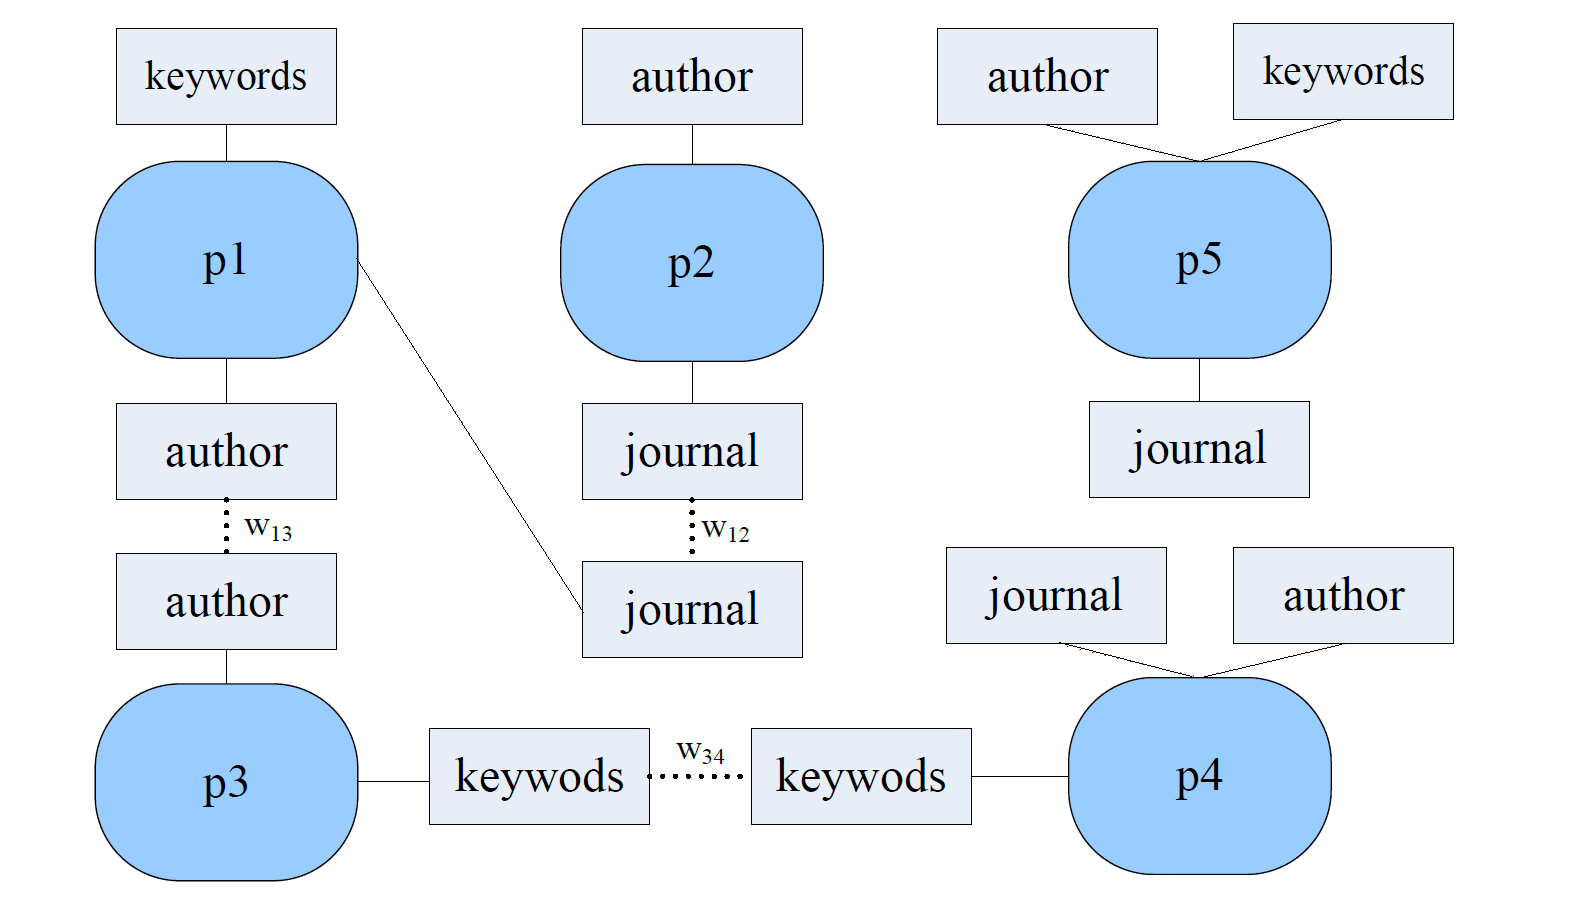
\includegraphics[width=\linewidth]{attr}
  \caption{特征关系图示意}
  \label{fig:attr}
\end{figure}

在特征关系图算法中主要利用节点之间的联通性,对于给定的特征关系图 $ G= \left ( V,E\right ) $,定义$ S(v_{i}) $为与$ v_{i} $相连接的文献节点集合,则得到从$ v_{i} $到$ v_{j} $的随机游走概率$ Pr\_Score\left ( v_{i},v_{j}\right ) $的值为:
\begin{equation}
\label{eq:pr}
Pr\_Score\left ( v_{i},v_{j}\right )=1+\frac{1}{d\left ( v_{i}\right )} \sum_{v\in s\left ( v_{i}\right )}^{}Pr\_Score\left ( v,v_{j}\right )
\end{equation}

其中$d\left(v_{i}\right)$是节点$v_{i}$ 的节点度数。公式\ref{eq:pr}是一个经典的随机游走模型\cite{aldous1989lower},本文用该公式计算从一个文献顶点$ v_{i} $经过一系列路径到达特定顶点 $v_{j}$ 的游走概率。

经上述分析,将文献集合转化成特征关系图,可以将文献实体间的潜在连通性直观的计算出来。本文以基于图划分的策略来实现基于特征关系图的消歧方法,在实现中先将每篇文献转化为图中的结点,计算所有结点(文献)间每维特征的相似性,如果相似度大于阈值(不同的特征阈值不同),则将两点之间加一条边,不必再计算其他文献特征。之后直接利用图的连通性分割为k个最大连通子图。该方法对文献间的相似度要求相对较高,必须达到很高的值才能在两篇文献节点间加一条边,否则会使消歧的准确度降低。完成特征关系图的构建之后,依据图的连通性,求特征关系图的每个连通子图,得到的每个连通子图就是最终的消歧聚类结果。具体算法如算法\ref{alg:conn}所示。

\begin{algorithm}  
  \caption{基于特征关系图的连通子图消歧算法}
  \label{alg:conn}  
  \begin{algorithmic}[1] %每行显示行号  
    \Require A list of papers $ P=\left\{p1,p2,\cdots\right\} $ and all they contain the same name "AAA" 
    
$\delta$ : the given threshold
    \Ensure The connected\_components of Graph
    \Function {DIS\_BY\_GRAPH}{}
    \State create a graph G with the nodes number of $\left | P\right |$
    \For{each node $p_{i}$ ,and $p_{i} \in P$} % For 语句,需要和EndFor对应
      \For{each $p_{j} \in G$ ,and $p_{i} \neq p_{j}$} % For 语句,需要和EndFor对应
        \State Compute the similarity of paper feature: $fsim\left(p_{i},p_{j}\right)$
        \If{$fsim\left(p_{i},p_{j}\right) > \delta$}
        \State $G.add\_edge \left(p_{i},p_{j}\right)$

        \State $weight=fsim\left(p_{i},p_{j}\right)$
        \EndIf
      \EndFor
    \EndFor
    \State \Return{G.connected\_components \#连通子图}  
    \EndFunction    
  \end{algorithmic}  
\end{algorithm}


\section{Experiment}
在本节的实验中使用 Python平台来构建特征关系图,测试数据集使用第三章介绍的数据集。本节实验了基于连通子图的消歧方法,文中综合使用了合作者、期刊、关键词、标题与摘要五种文献特征属性,文献特征相似度阈值设定为 1.5,之后将图的连通子图作为最终聚类结果。

在实验中发现,文献之中存在比较脏的数据,这些数据严重拖累了构建连通子图的效率,在没有去除这些脏数据的情况下,准确率很低。于是尝试去除这些比较脏的数据,对于其中存在成百上千个合著者的文献采取了截断处理,只保留前几十个合著者信息,对于作者机构信息,由于没有好的文本处理方式,我们采用了简单的文字相似度比较,用来比较两个机构是否是同一机构。机构存在与作者任命相同的问题,表示方法众多,简写方式不统一,这给实验造成了很大的麻烦,导致最后的准确率一直得不到提高,徘徊在0.35左右。

由于此方法对文献相似阈值比较敏感,在文献的消歧测试中对不同的阈值也做了尝试,当文献相似度阈值设置过低时,导致消歧准确率下降,阈值过高,又导致消歧召回率降低明显,在1.5时消歧结果的F-measure 得到最好的结果,因为需要更高的准确度,最终文献间的相似度阈值设为 1.5。

基于划分连通图的消歧算法虽然最大限度的利用了节点的连通性,但对于特殊文献作者情形,如论文数目比较少且彼此间联系少的情形,消歧结果的召回率还不是很理想,这将是以后努力的方向。



\section{Conclusion}
本文提出了一种基于特征关系图的作者消歧方法。在文献作者消歧问题中引入了特征关系图的概念,将作者消歧问题转化成图的划分问题,同时也使用了基于图的连通属性来计算文献节点间的附加概率。基于连通子图划分的消歧方法,充分利用文献结点的连通性,取得了最好的消歧识别实验结果,相比简单的层次聚类算法,平均准确率有了很大的提升。特征关系图的消歧方法相比较于传统的基于合作者网络的方法,充分利用了其他属性特征,其中基于图的连通子图划分的方法取得了很好的效果。

%%
%% The next two lines define the bibliography style to be used, and
%% the bibliography file.
\bibliographystyle{ACM-Reference-Format}
\bibliography{project}
\end{document}
\endinput
%%
%% End of file `sample-sigchi.tex'.
